\section{Problem 1 – Linear Algebra – LU decomposition}

\paragraph{Question 1}
A lower triangular matrix $M$ has $M_{i,j} = 0$ for $i < j$.
Let $L, L' \in \mathbb{R}^{n\times n}$ be a lower triangular matrices.
Let's look closer at entries above diagonal of $LL'$, i.e. $(LL')_{i,j}$ for $i<j$:
\begin{equation*}
    (LL')_{i,j} = \sum_{k=1}^{n} L_{i,k} \cdot L'_{k,j}
\end{equation*}
Every item of the summation yields either $i<k$ or $k<j$.
Thus,  $(LL')_{i,j} = 0$ for $i<j$.

The same another way:
\begin{align*}
    (LL')_{i,j} &= \sum_{k=1}^{n} L_{i,k} \cdot L'_{k,j} \\
                &= \sum_{k=1}^{j-1} L_{i,k} \cdot L'_{k,j} + \sum_{k=j}^{n} L_{i,k} \cdot L'_{k,j} \\
                &= \sum_{k=1}^{j-1} L_{i,k} \cdot 0 + \sum_{k=j}^{n} 0 \cdot L'_{k,j} \\
                &= 0
\end{align*}


\paragraph{Question 2}
Let $L, L' \in \mathbb{R}^{n\times n}$ be a \emph{unit} lower triangular matrices, i.e $L_{i,j} = L'_{i,j} = 1$ for $i = j$.
We know from Q1, that $LL'$ is lower triangular.
Let's examine diagonal items, $(LL')_{i,i}$:
\begin{equation*}
    (LL')_{i,i} = \sum_{k=1}^{n} L_{i,k} \cdot L'_{k,i}
            = L_{i,1} L'_{1,i} + L_{i,2} L'_{1,i} + \dots + L_{i,i} L'_{i,i} + \dots + L_{i,n} L'_{n,i} = 1
\end{equation*}


\paragraph{Question 3}
Inverse of a unit lower triangular matrix is also unit lower triangular.
So, we need to find only one entry of the inverse of $L1$, such that:
\begin{equation*}
L_1 L_1^{-1} =
\begin{pmatrix}
1 & 0\\
2 & 1
\end{pmatrix}
\cdot
\begin{pmatrix}
1 & 0\\
x & 1
\end{pmatrix}
=
\begin{pmatrix}
1 & 0 \\
0 & 1
\end{pmatrix}
\end{equation*}
Obviously, $x=-2$. Simillary, $L_2$:
\begin{equation*}
L_2 L_2^{-1} =
\begin{pmatrix}
1 & 0 & 0 \\
2 & 1 & 0 \\
3 & 2 & 1
\end{pmatrix}
\cdot
\begin{pmatrix}
1 & 0 & 0 \\
a & 1 & 0 \\
b & c & 1
\end{pmatrix}
=
\begin{pmatrix}
1 & 0 & 0 \\
0 & 1 & 0 \\
0 & 0 & 1
\end{pmatrix}
\end{equation*}
Here, $a = -2$, $b = 1$, $c = -2$.

\paragraph{Question 4}
% Prove that $LU$ decomposition of a matrix is unique if $L$ is \emph{unit} lower triangular matrix.
Prove that if $A$ has two different LU decomposition, that is $A = LU = L_1U_1$ and $L, L_1$ are lower \emph{unit} matrices, then $L=L_1$ and $U=U_1$.

Assume that inverses of $U, U_1$ exist.
Start with $A= LU = L_1 U_1 = A$ and multiply right-hand by $U^{-1}$ and left-hand by $L_1^{-1}$:
\begin{align*}
    LU &= L_1 U_1 \\
    L_1^{-1} L U U^{-1} &= L_1^{-1} L_1 U_1 U^{-1} \\
    L_1^{-1} L  &=  U_1 U^{-1} \\
\end{align*}
We know from (Q2) that left-hand side of the last equation is lower unit triangular matrix.
In similar manner, we can show that right-hand is upper triangular.
Lower and upper triangular matrices can be equal iff they are both diagonal.
Moreover, since $L_1^{-1} L$ has ones on diagonal, so $U_1 U^{-1}$ must have.
We conclude:
\begin{align*}
     L_1^{-1} L = Id = U_1 U^{-1}
\end{align*}
That is, $L = L_1$ and $U = U_1$.
 

\section{Problem 2 – Automata Theory}
\paragraph{Question 1}
$a^*b^*a^*$

\paragraph{Questions 2 - 5}
See Fig. \ref{fig:w2016-w-2-2} - \ref{fig:w2016-w-2-5}

\begin{figure}[!h]
    \centering
    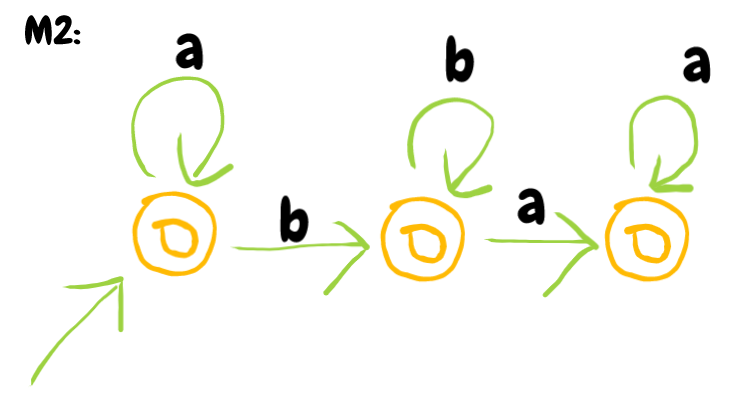
\includegraphics[scale=0.5]{data/2016-W-2-2.png}
    \caption{Question 2}
    \label{fig:w2016-w-2-2}
\end{figure}

\begin{figure}[!h]
    \centering
    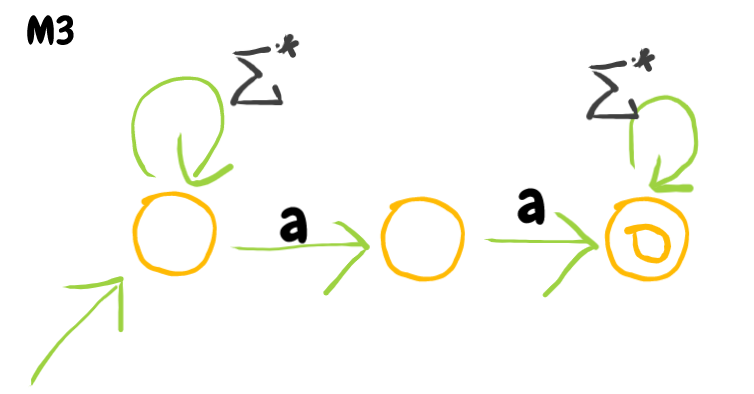
\includegraphics[scale=0.5]{data/2016-W-2-3.png}
    \caption{Question 3}
    \label{fig:w2016-w-2-3}
\end{figure}

\begin{figure}[!h]
    \centering
    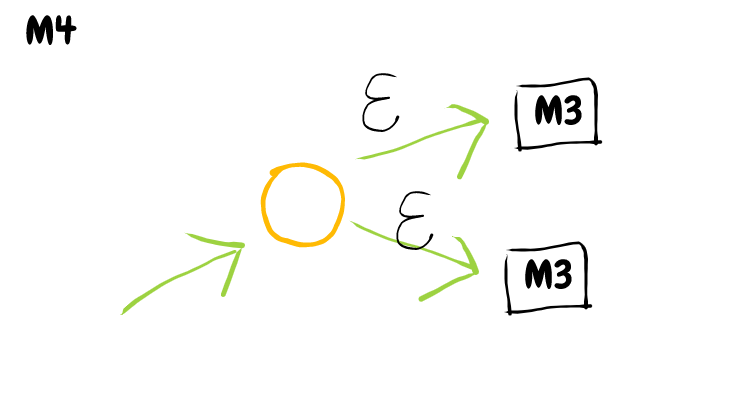
\includegraphics[scale=0.5]{data/2016-W-2-4.png}
    \caption{Question 4. One of the boxes should be labeled $M_1$.}
       \label{fig:w2016-w-2-4}
\end{figure}

\begin{figure}[!h]
    \centering
    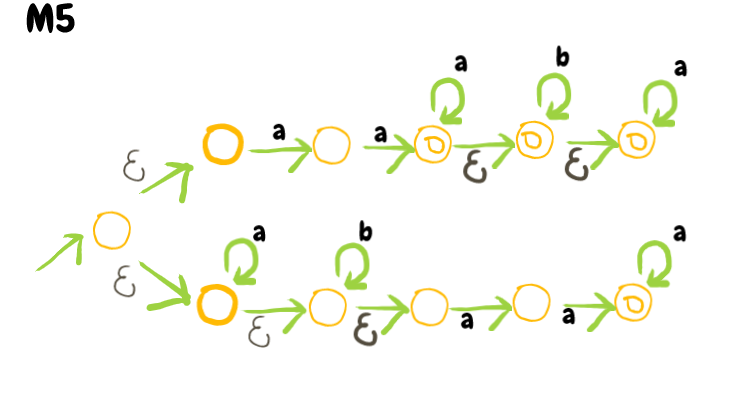
\includegraphics[scale=0.5]{data/2016-W-2-5.png}
    \caption{Question 5. $L(M_5)$ contains $aa$ and is of form of $aaa^* b^* a^* + a^* b^* aaa^*$}
       \label{fig:w2016-w-2-5}
\end{figure}



\section{Problem 3 – AVL Tree}

\paragraph{Question 1}
Easy  % tikz hf

\paragraph{Question 2}
Minimum height of BST with $n$ nodes is $\lfloor log_2n\rfloor$.
Maximum height: $n-1$.

\paragraph{Question 3}
AVL tree with $7$ nodes has min. height of $2$ (full binary tree), and max. height of $3$. See Fig. \ref{fig:2016-3-3avl}
\begin{figure}[!h]
    \centering
    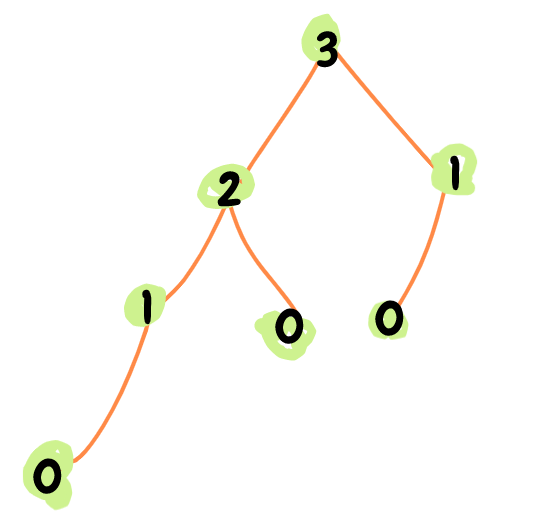
\includegraphics[width=50pt]{data/2016-W-3-3.png}
    \caption{Max. height AVL Tree with 7 nodes.
    Numbers in nodes indicate height of a tree rooted in the node. }
    \label{fig:2016-3-3avl}
\end{figure}

\paragraph{Question 4}
Just $\lfloor log_2n\rfloor$ – it's a full binary tree.


\paragraph{Question 5}
Show that the height of a balanced binary tree (AVL) with $n$ nodes is no more than $2log_2n$.

Let's consider the smallest possible AVL trees wrt number of nodes.
Let $N(h)$ indicate minimum number of nodes in a balanced tree of height $h$.
The minimum tree of $n$ nodes and height $h$ consists of a root, a \emph{minimum} subtree of of height $h-1$ and a \emph{minimum} subtree of height $h-2$:
\begin{align*}
    n = N(h) &= 1 + N(h-1) + N(h-2) \\
            &\geq 1 + 2 \cdot N(h-2) && \text{because } N(h) > N(h-1) \\ 
            &> 2 \cdot N(h-2) \\
            &\geq 2^{\frac{h}{2}}
\end{align*}
Taking log both sides: $h \leq 2\cdot log_2(n)$.


\section{Problem 4 – Logic Circuit Design}
\paragraph{Question 1}
\begin{enumerate}
    \item OR($x, y$) = $majority(0, x, y)$
    \item AND($x, y$) = $majority(1, x, y)$
    \item XOR($x, y$) = AND( OR($x,y$), NOT( AND($x, y$) ) = $majority[1, majority(0,x,y) , not\:majority(1, x, y)]$
\end{enumerate}
XOR is "$2$-$M_3$-level".

\paragraph{Question 2}
Classic $1$-bit full adder. 
Just draw a table and then depict the circuit.
Let $a,b,c_{in}$ be inputs.
\begin{align*}
S = a\veebar b \veebar c_{in}    &&
C = (a\land b) \lor (c_{in} \land (a \lor b))
\end{align*}
$S$ yields $4$~-~$M_3$ level (2x XOR).
$C$ yields $3$~-~$M_3$ level (OR with 2-level AND).
Thus, $FA_1$ has $4$~-~$M_3$ level.

Bonus: $C = majority(c_{in}, a,b)$.
Thanks Igor!

\paragraph{Question 3}
Connect $4$ $FA_1$ in series.
It's $M_3$ level is $4\cdot4 = 16$. 

\paragraph{Question 4}
Classic $4$-bit multiplier (google for images).
Connect three $4$-bit adders in series and try not to get messed with connections.
$M_3$ level is: $3\cdot 16 + 8\cdot 1$: each of three $FA_4$ has level $16$ and there's one level of $8$ AND gates preceding $FA_4$'s.